\documentclass{standalone}
\usepackage{tikz}
\usetikzlibrary{arrows.meta, positioning}

\tikzset{
    red node/.style={circle, draw, fill=red!20, minimum size=6mm},
    blue node/.style={circle, draw, fill=blue!20, minimum size=6mm},
    arrow/.style={->, line width=0.6pt},
}

\begin{document}
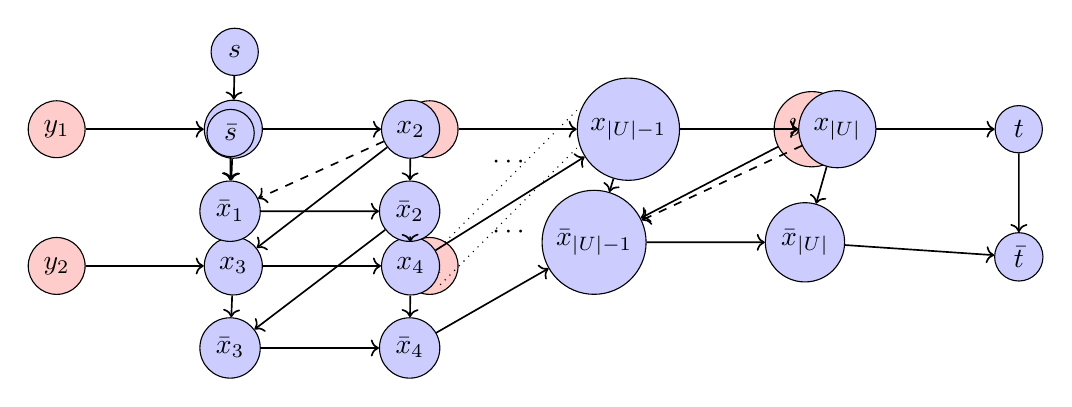
\begin{tikzpicture}[scale=0.8, node distance=1cm and 1.5cm]

    % Left side nodes
    \node[red node] (y1) {$y_1$};
    \node[red node, below=of y1] (y2) {$y_2$};
    \node[red node, right=4cm of y1] (y3) {$y_3$};
    \node[red node, below=of y3] (y4) {$y_4$};
    \node[red node, right=4cm of y3] (yC) {$y_{|C|}$};

    \node[blue node, right=of y1] (x1) {$x_1$};
    \node[blue node, right=of x1] (x2) {$x_2$};
    \node[blue node, right=of y2] (x3) {$x_3$};
    \node[blue node, right=of x3] (x4) {$x_4$};
    \node[blue node, right=of y3] (xC1) {$x_{|U|-1}$};
    \node[blue node, right=of xC1] (xC) {$x_{|U|}$};

    \node[blue node, below left=0.5cm and -0.5cm of x1] (xbar1) {$\bar{x}_1$};
    \node[blue node, right=of xbar1] (xbar2) {$\bar{x}_2$};
    \node[blue node, below left=0.5cm and -0.5cm of x3] (xbar3) {$\bar{x}_3$};
    \node[blue node, right=of xbar3] (xbar4) {$\bar{x}_4$};
    \node[blue node, below left=0.5cm and -0.5cm of xC1] (xbarU1) {$\bar{x}_{|U|-1}$};
    \node[blue node, right=of xbarU1] (xbarU) {$\bar{x}_{|U|}$};

    \node[blue node, above left=0.5cm and -0.5cm of x1] (s1) {$s$};
    \node[blue node, above left=0.5cm and -0.5cm of xbar1] (s2) {$\bar{s}$};

    \node[blue node, right=of xC] (t) {$t$};
    \node[blue node, below=of t] (tbar) {$\bar{t}$};

    % Connections
    \draw[arrow] (s1) -- (x1);
    \draw[arrow] (s2) -- (xbar1);
    \draw[arrow] (x1) -- (x2);
    \draw[arrow] (x2) -- (x3);
    \draw[arrow] (x3) -- (x4);
    \draw[arrow] (x4) -- (xC1);
    \draw[arrow] (xC1) -- (xC);
    \draw[arrow] (xC) -- (t);
    \draw[arrow] (t) -- (tbar);

    \draw[arrow] (xbar1) -- (xbar2);
    \draw[arrow] (xbar2) -- (xbar3);
    \draw[arrow] (xbar3) -- (xbar4);
    \draw[arrow] (xbar4) -- (xbarU1);
    \draw[arrow] (xbarU1) -- (xbarU);
    \draw[arrow] (xbarU) -- (tbar);

    \draw[arrow] (y1) -- (x1);
    \draw[arrow] (y2) -- (x3);
    \draw[arrow] (y3) -- (xC1);
    \draw[arrow] (yC) -- (xbarU1);

    \draw[arrow] (x1) -- (xbar1);
    \draw[arrow] (x2) -- (xbar2);
    \draw[arrow] (x3) -- (xbar3);
    \draw[arrow] (x4) -- (xbar4);
    \draw[arrow] (xC1) -- (xbarU1);
    \draw[arrow] (xC) -- (xbarU);

    \draw[arrow, dashed] (x2) -- (xbar1);
    \draw[arrow, dashed] (x4) -- (xbar2);
    \draw[arrow, dashed] (xC) -- (xbarU1);

    \draw[dotted] ([yshift=3mm]x4.east) -- node[above] {$\cdots$} ([yshift=3mm]xC1.west);
    \draw[dotted] ([yshift=-3mm]x4.east) -- node[below] {$\cdots$} ([yshift=-3mm]xC1.west);

    % Dashed connection for y_C
    \draw[arrow, dashed] (yC) -- (xC);
\end{tikzpicture}
\end{document}